\section{Classification of Graph Data Generators}
\label{sec:classification}

The graph data generators can be classified according to distinct criteria. For example, paper~\cite{DBLP:conf/sdm/ChakrabartiZF04} introduces two categories:

\begin{itemize}
  \item \emph{Degree-based generators}: Given a (customarily power law) degree distribution, these generators (e.g., Barabasi-Albert model~\cite{Barabasi99emergenceScaling}) attempt to produce a graph matching the above distribution. However, they do not provide any insights about the graph or ignore the matching of other parameters such as for instance small diameter, eigenvalues and so on.
  \item \emph{Procedural generators}: These generators (e.g., R-MAT~\cite{DBLP:conf/sdm/ChakrabartiZF04}) try to find simple mechanisms to generate graphs that match a property of the real graphs and, typically, the power law degree distribution.
\end{itemize}

Paper~\cite{Chakrabarti:2006:GML:1132952.1132954} introduces five categories of graph models (examples are further described below):
\begin{itemize}
  \item \emph{Random graph models} (e.g., Erd\"{o}s-R\'{e}nyi~\cite{Erdos:1960}) generated by a random process,
  \item \emph{Preferential attachment models} (e.g., Barabasi-Albert model) which try to model the power law from the preferential attachment viewpoint,
  \item \emph{Optimization-based models} (e.g., HOT model~\cite{PhysRevLett.84.2529}) resulting from the idea that power laws can result from resource optimizations and tolerance to risks,
  \item \emph{Tensor-based models} (e.g., R-MAT) targeting a trade-off between low number of model parameters and efficiency, and
  \item \emph{Internet-specific models} corresponding to hybrids using ideas from the other categories in order to suit the specific features of the graphs.
\end{itemize}

\paragraph{Erd\"{o}s-R\'{e}nyi} One of the first and still very popular approaches with lots of variations and modifications is the random graph model proposed in~\cite{Erdos:1960}. Given a positive integer $n$ and a probability value $0 \leq p \leq 1$, the graph $G(n,p)$ is an undirected graph on $n$ vertices whose edges are chosen s.t. for all pairs of vertices $u,v$ there is an edge $(u,v)$ with probability $p$.

\paragraph{Barabasi-Albert} The Barabasi-Albert (BA) model~\cite{Barabasi99emergenceScaling} proposes that structure emerges in network topologies as the result of two processes -- growth and preferential attachment. The BA model starts with a small set of nodes and grows the network as nodes and edges are added over time. Preferential attachment is based on the idea that the probability of connecting to a node is proportional to the current degree of that node (i.e., ``the rich get richer'').

\paragraph{HOT} The highly optimized tolerance (HOT)~\cite{PhysRevLett.84.2529} model is introduced  using a ``forest fire'' example as follows: Suppose we have a forest which is prone to forest fires. Each portion of the forest has a different chance of starting the fire. We wish to minimize the damage by assigning (a limited amount of) resources such as firebreaks at different positions in the forest. More precisely, we have $n$ possible events, each with an associated probability $p_i, 1 \le i \le n$. Each event can lead to some loss $l_i$, which is a function of the resources $r_i$ allocated for that event $(l_i = f (r_i))$, whose total number is limited ($\sum_i r_i \le R$ for some given $R$). The aim is to minimize the expected cost $\sum_i p_i l_i$. The authors show that resource placement is related to the probability distribution $p_i$ by a power law and the probability of events which cause a loss greater than some value $k$ is related to $k$ by a power law too.


\paragraph{R-MAT} The R-MAT (Recursive MATrix)~\cite{DBLP:conf/sdm/ChakrabartiZF04} model can be used to create graphs with community structure, power law degree distributions, and a small diameter. It generates weighted, directed and bipartite graphs. Graph generation is modeled with a matrix recursion procedure in which the adjacency matrix (empty at the beginning) is recursively subdivided into four equal-sized partitions and edges are distributed across the partitions with unequal probabilities.
\\



...


%~\cite{Gray:1992:BHD:530588}

Ideas to describe:

\begin{itemize}
  \item Domain-specific - predefined schema and domain knowledge - vs. application-specific~\cite{Tay2011}
  \item Use-case driven
  \item Query-centric vs. workload-driven~\cite{gMark}
  \item Language-specific (the document and query design is specifically laid out to test common language constructs, operator constellations, and data access patterns)~\cite{Schmidt2010}
  \item Application benchmarks attempt to predict the behaviour of a system on
certain classes of application by testing an example (or select examples) of that
class.
  \item Analytical benchmarks attempt to determine the presence or absence of cer-
tain performance related features, e.g., the presence of a query optimiser.
\end{itemize}

...

In Figure~\ref{fig:classification} ...

\begin{figure}
\centering
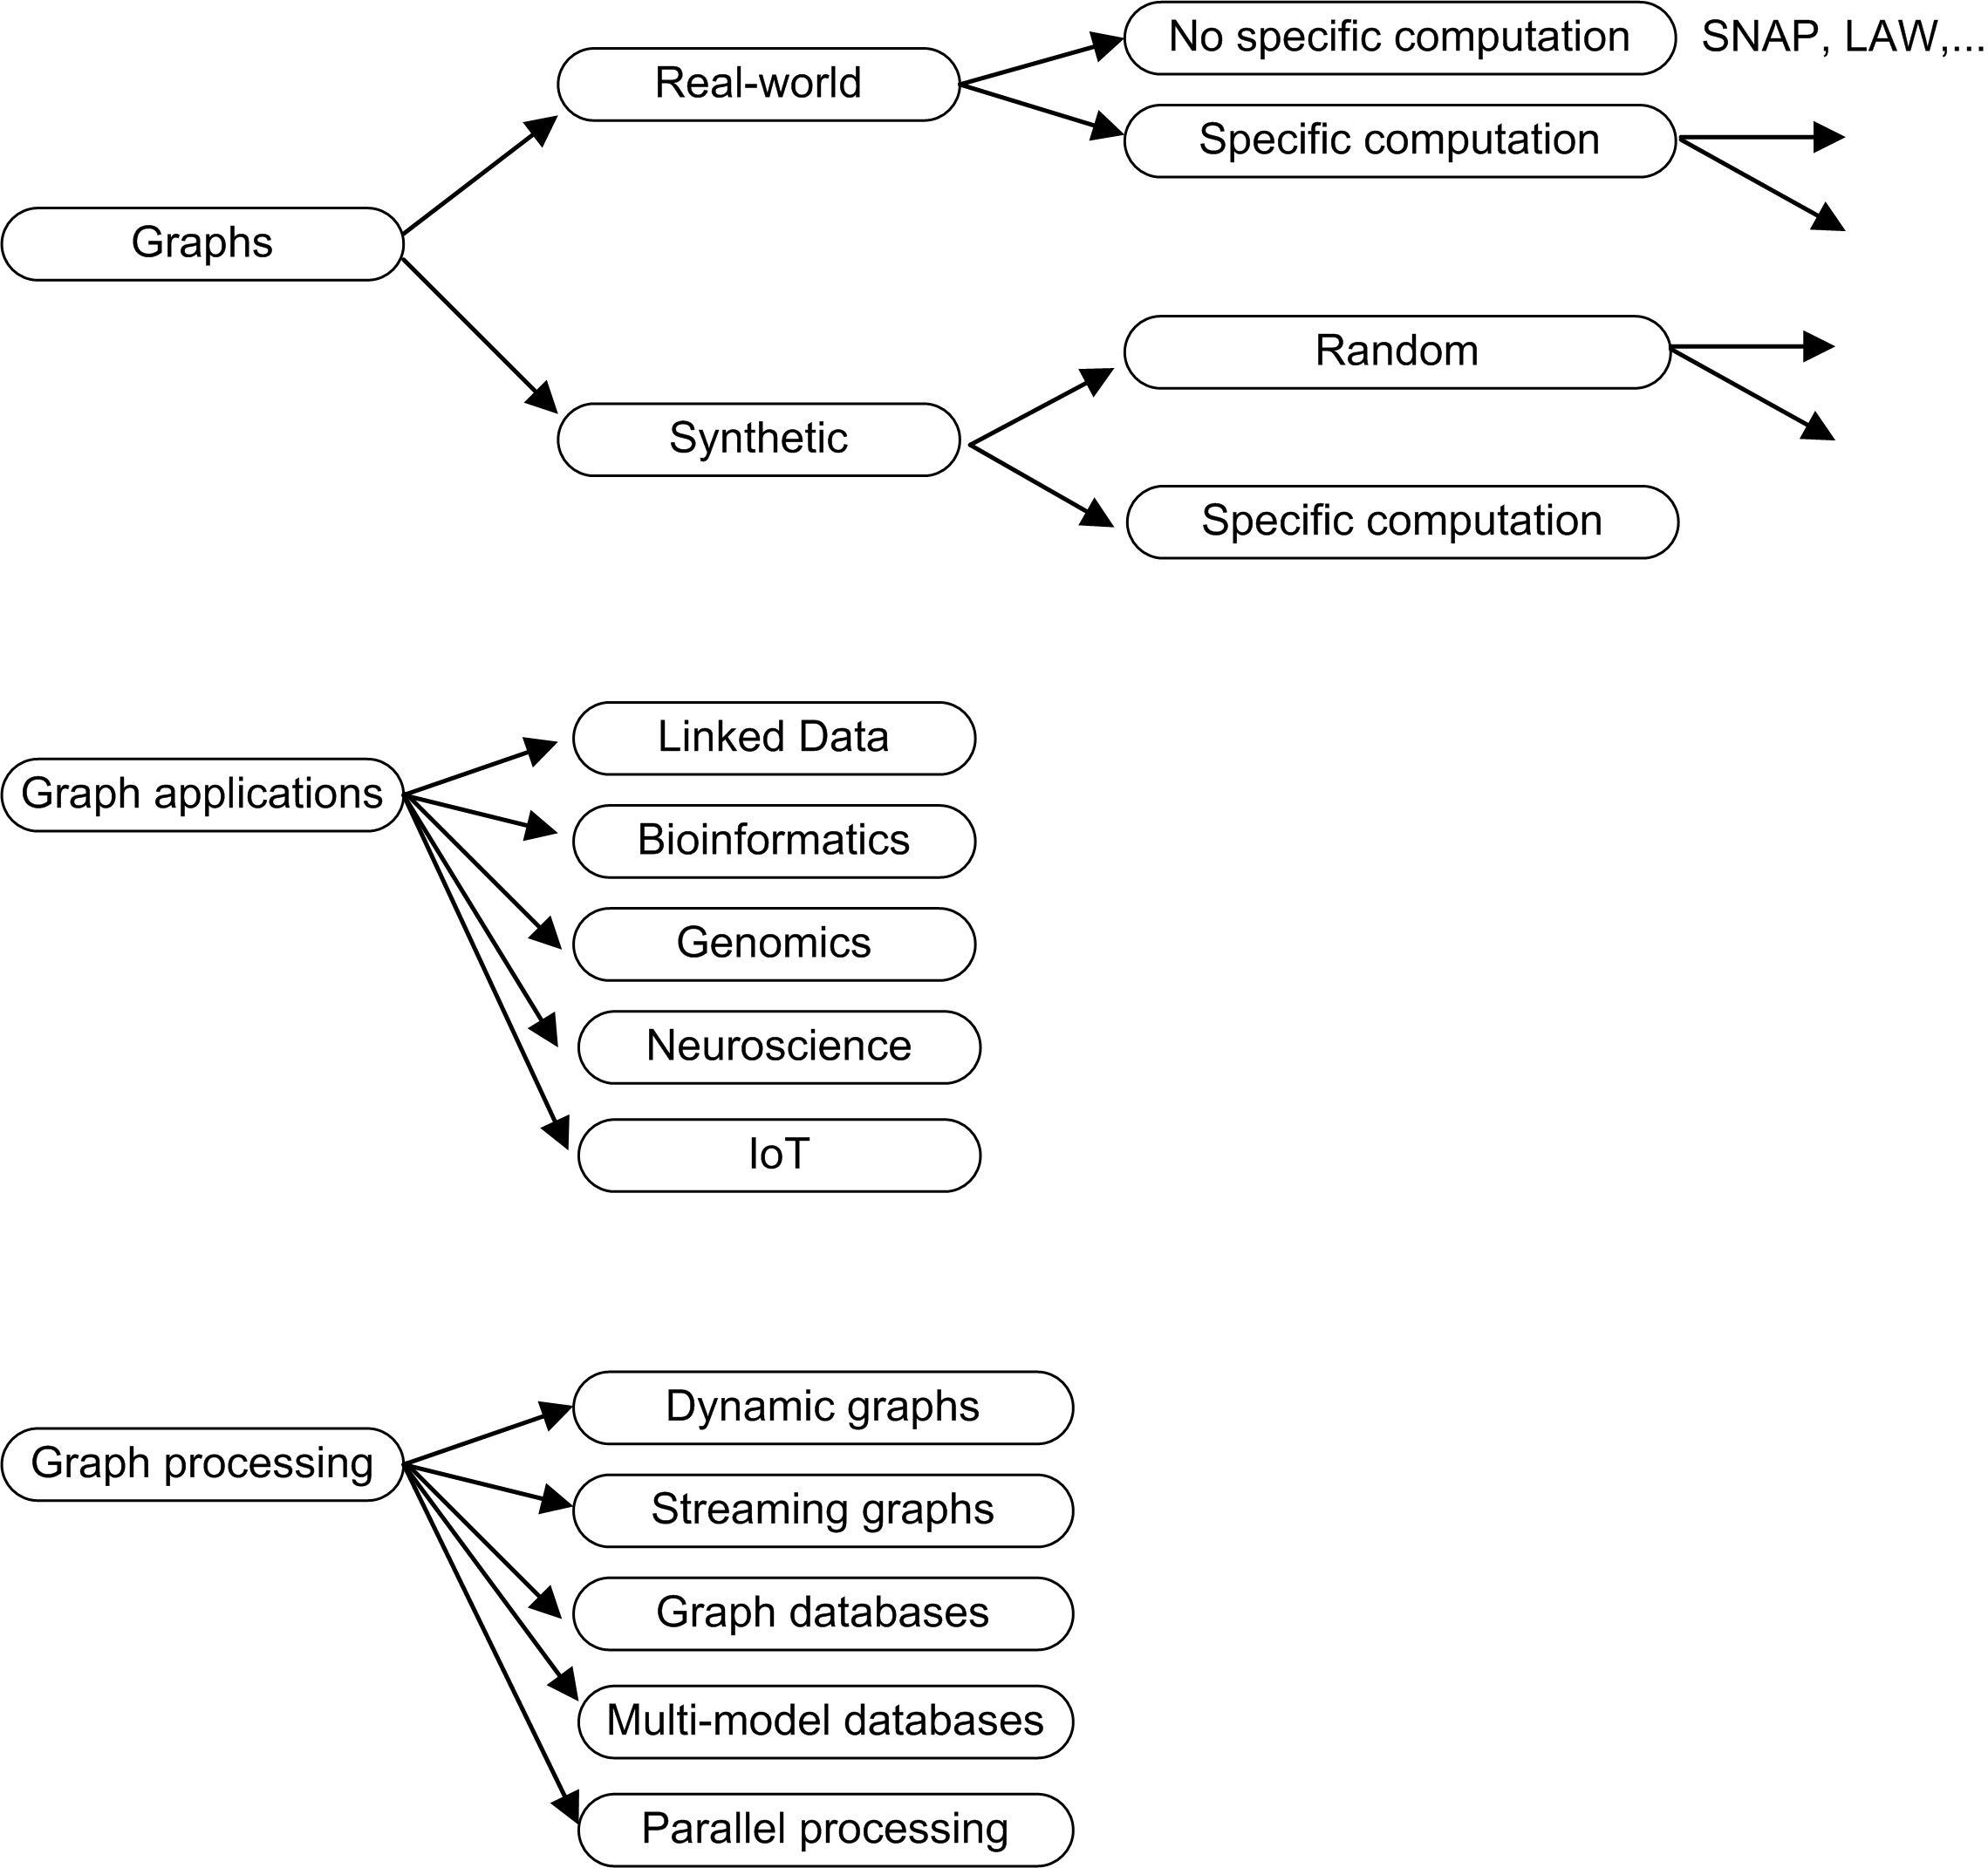
\includegraphics[width=0.8\textwidth]{classification.png}
\caption{Classification of graph data generators}
\label{fig:classification}
\end{figure}
